% \paragraph{}
% Un système de gestion des informations géotechiques s'avère incontournable
% dans un environnement de géoscience. Beaucoup d'universités et d'entreprises 
% privées ainsi que l'état dans certains pays à travers le monde se sont déjà 
% penchés sur la question. 
% \paragraph{}
% Les résutats divergent sur quelques détails à propos des technologies utilisées mais 
% l'objectif est généralement le même: 
% constituer une base de données renseignée regroupant tous les points (sondages, essais
% in situ ou en laboratoire) améliorant la connaissance des caractéristiques géomécaniques des
% formations d'une zone.
% Par exemple, dans les Caraïbes, plus précisement sur l'Ile de Cayenne, un tel système a permis
% de mieux appréhender les types de problèmes
% spécifiques au site, et donc de mieux dimensionner les campagnes de reconnaissance
% géotechniques, aussi bien sur le plan technique que financier
% \cite{cayenne}.
% \par 
% L'une des faiblesses de certains projets est l'utilisation des outils de Microsoft
% qui ne semblent pas assez 
% adéquats. Ils sont trop génériques, ce qui empêche un stockage intelligent des données géotechniques
% \cite{antoljak2012subsurface}.

% %......................

% \paragraph{}D'autres se basent de préférence sur la conception d'une architecture d'information 
% géotechnique à l'aide de services Web
% \cite{zimmermann2003design}.
% Cette architecture d'information a été implémentée à Los Angeles afin de permettre les échanges 
% d'informations géotechniques accessibles pour tous. Les avantages apportés par une telle 
% application pourraient tant se sentir pour des études concernant les risques sismiques que pour 
% une meilleure approche lors des estimations effectuées par des compagnies d'assurance. 

% \paragraph{}
% Au Canada, plusieurs projets identiques ont vu le jour, notemment l'élabora\-tion d'une base 
% de données géoscientifiques dans le but d’aider à la finalisation de la 
% cartographie des dépôts en surface et en subsurface
% \cite{russell1996regional}.

% %............................

% \paragraph{}
% En 2011, un séisme a frappé la région de Canterbury (Nouvelle-Zélande). Une base de données en ligne a été développée pour
% la reconstruction de Christchurch à la suite du tremblement de terre:
% La base de données géotechniques de Canterbury (CGD). Elle
% a été conçue comme un référentiel consultable pour le partage d'informations géotechniques existantes et nouvelles
% ainsi que des applications géotechniques de soutien pour les autorisations de construction. En mars
% 2015, la base de données contient plus de 18000 enregistrements d'essais de pénétration de cône, 4000 forages, 1000
% piézomètres accompagnés de registres de surveillance des eaux souterraines, 6000 enregistrements de tests de laboratoire
% plus d'autres données. 

% \par
% Le CGD (Figure: \ref{fig:canterbury}) a été conçu comme un référentiel consultable pour les informations géotechniques existantes et nouvelles
% ainsi que des applications géotechniques de soutien pour les autorisations de construction. Tandis que
% les données sont principalement utilisées pour la conception géotechnique de l'amélioration du sol, la fondation du bâtiment,
% réparations, fondations de nouveaux bâtiments et conception géotechnique pour les réparations d'infrastructures, il peut
% également être utilisé à des fins plus stratégiques tel que l'aide à la récupération pour de futures
% catastrophes naturelles.
% \cite{scott2015benefits}

% \begin{figure}[t]
%     \centering
%     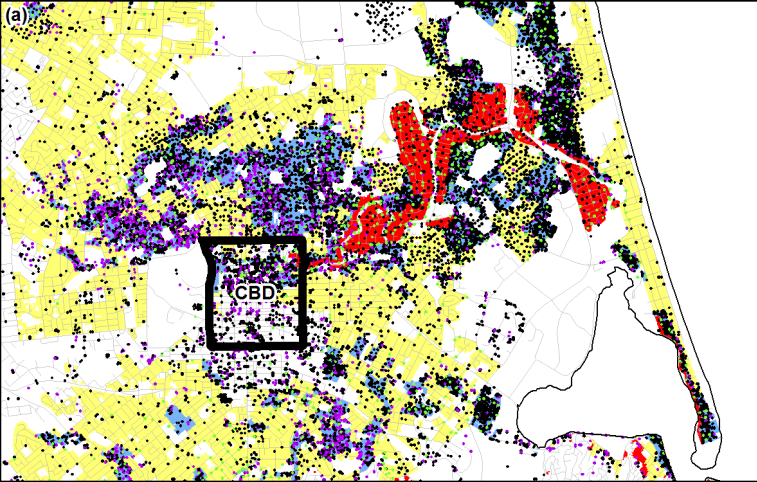
\includegraphics[width=1\textwidth]{images/Contexte/cgd.png}
%     % \caption{Visualisation des résultats de la base de données de Canterbury \cite{scott2015benefits}.}
%     \label{fig:canterbury}
% \end{figure}

% %............................

% \paragraph{}
% L'Afrique ne fait pas exception à la liste des multiples endroits ayant adopté l'idée
% de concevoir des bases de données géotechniques.
% Par exemple, celle de la ville de Tunis (Tunisie) est orientée vers la cartographie géotechnique.
% \par
% Le modèle choisi a permis, après une analyse
% pré1iminaire très importante, une description globale et
% totale de toutes les données géologiques et géotechniques collectées sur le site de Tunis. Il
% assure, de plus, une indépendance physique et logique, un partage des données (une même donnée accessible  
% par plusieurs programmes), une non-redondance des données, une grande facilité des relations
% entre fichiers indépendants, une intégrité (validité)
% totale des données. 
% \textit{S'y ajoutent une souplesse remarquable d'interrogation de TUNIS-DATA-BANK
% assurée par l'emploi d'un langage d'interrogation spécifique et l'utilisation des opérateurs et des connecteurs
% logiques, une automatisation totale des tâches de la
% phase de la manipulation de la base de données et une
% sécurité totale des fichiers.}
% \cite{mongereau1988conception}

% %..................
% \paragraph{} 
% Parmi les BDD géotechniques gouvernementales (Figure:\ref{fig:BDG}), la Base de Données Géotechniques
% (BDG) du gouvernement canadien, plus précisément le
% ministère des transports du Québec, et le "Geotechnical Web Mapping App" (Figure:\ref{fig:wash}) se font remarquer
% de par leur simplicité et leur efficacité. Ces deux systèmes présentent les sondages, les forages ainsi que les 
% propriétés des sols et des roches dans plusieurs zones de ces deux pays.
% Un webmap est utilisé pour faciliter la visualisation de ces données.
% De plus, le résultat de chaque étude est mis à la disposition du public
% via un lien PDF.

% \begin{figure}[t]
%     \centering
%     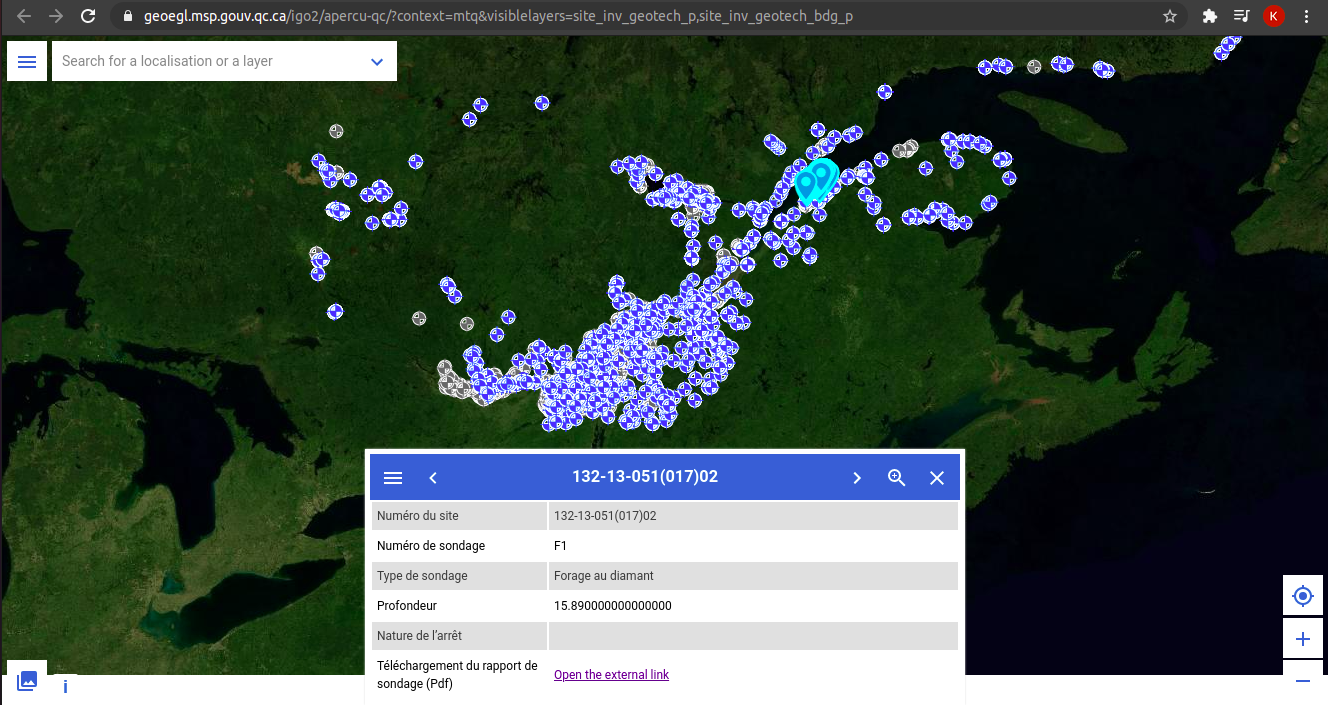
\includegraphics[width=1\textwidth]{images/Contexte/bdg.png}
%     % \caption{Webmap de la BDG du gouvernement du Canada \cite{canadagov}}
%     \label{fig:BDG}
% \end{figure}
% \begin{figure}[t]
%     \centering
%     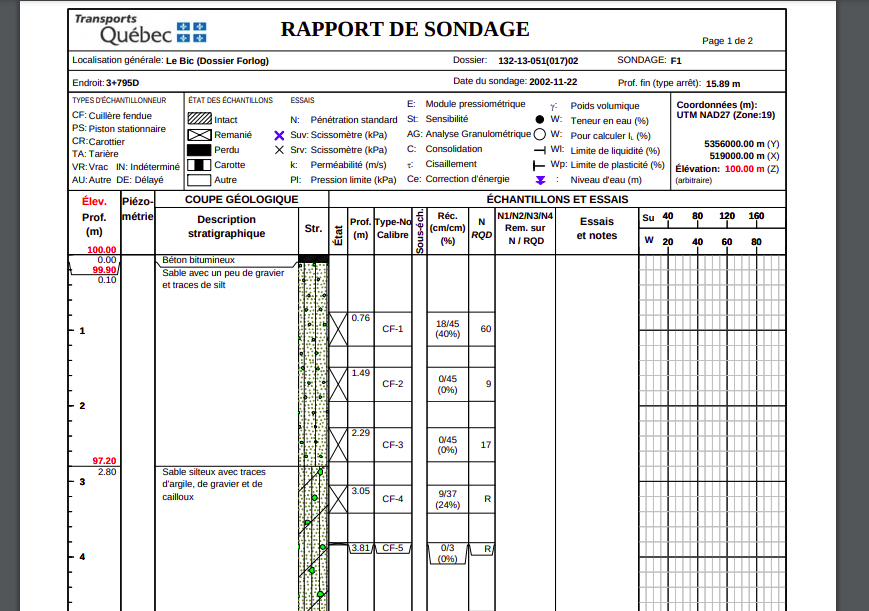
\includegraphics[width=1\textwidth]{images/Contexte/pdf_bdg.png}
%     \caption{PDF d'un rapport de sondage de la BDG du gouvernement du Canada \cite{linkpdfcanada}}
%     \label{fig:PDF_BDG}
% \end{figure}
% \begin{figure}[t]
%     \centering
%     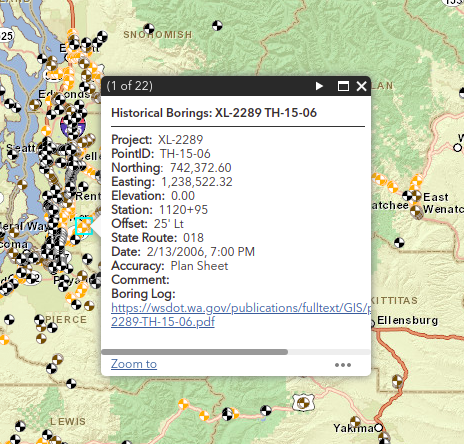
\includegraphics[width=1\textwidth]{images/Contexte/wash.png}
%     \caption{Information sur une étude spécifique dans le Geotechnical Web Mapping App \cite{map1}}
%     \label{fig:wash}
% \end{figure}

% \paragraph{}
% L’implémentation de tous ces SIG par des organismes internationaux résulte à des données considérées 
% comme étant le système d’archivage officiel dans leur domaine de spécialité.
% Le rythme de migration de ces données dans le SIG Web connait une croissance exponentielle. 
% Quelques exemples sont donnés dans le tableau \ref{tab:someBDD}.
% \par
% Avec son mouvement vers le cloud et sur le Web, son intégration à l'information 
% en temps réel via l'Internet des objets, le SIG est devenu une plateforme 
% pertinente pour presque toutes les activités humaines - un système nerveux de 
% la planète. Alors que notre pays est confronté au problèmes de gestion et de vulgarisation 
% des données géotechiques, les SIG joueront un rôle de plus 
% en plus important et 
% fourniront un moyen de communiquer des solutions en utilisant le langage commun de 
% la cartographie.

% \par    
% \begin{table}
%         \centering
%         \begin{tabular}{|p{0.40\linewidth}|p{0.60\linewidth}|}
%         \hline
%                 \textbf{BDD} & \textbf{Fonctions} \\
%                 \hline
%                     British Geological Survey (BGS) créée par le
%                     Royaume-Uni&
%                     Fournisseur de données, 
%                     d’informations et de connaissances 
%                     géoscientifiques objectives britannique
%                          \\
%                 \hline
%                     SERNAGEOMIN (Figure:\ref{fig:chili}) créée par le
%                     Gouvernement du Chili&
%                     Génération 
%                     d'informations géologiques sur le territoire 
%                     chilien, ses dangers géologiques et sa mise 
%                     à disposition des citoyens
%                          \\
%                 \hline 
%                     La base de données géotechniques de Canterbury (CGD) créée par le
%                     Gouvernement de la Nouvelle Zélande&
%                     Génération 
%                     d'informations géologiques sur le territoire 
%                     chilien, ses dangers géologiques et sa mise 
%                     à disposition des citoyens
%                         \\
%                 \hline 
%                     DBG créée par
%                     Ministère des transports du Québec&
%                     - Présentaion des sondages
%                     - Présentaion des forages sous forme schématique
%                     - Présentaion des propriétés des sols et des roches
%                     - Présentaion de la qualité de l’eau souterraine
%                         \\
%                 \hline 
%                 GISOS créée par
%                 trois organismes: BRGM, INERIS, INPL-LAEGO&
%                     - Accès facile aux informations sur les forages
%                     - Accès aux mouvements de terrain
%                     - Accès aux mesures topographiques
%                     - Accès aux essais au laboratoire
%                         \\
%                 \hline 
%                 Base de données géotechniques, géodésiques
%                  et géophysiques dans les argiles du Trièves créée par
%                  le conseil général de l'Isère&
%                         -Mise à disposition des utilisateurs potentiels, scientifiques ou opérationnels des informations
%                         géotechniques, géodésiques et géophysiques.
%                        \\
%                 \hline 
%                 SIGPEG
%                 et géophysiques dans les argiles du Trièves&
%                         - Accès aux informations sur les données
%                         cartographiques, géophysiques, géotechniques, sur les puits forés
%                             \\
%                 \hline 
%         \end{tabular}
%         \caption{Présentation de quelques BDD géotechniques dans le monde} \label{tab:someBDD}
% \end{table}
% \par

% \begin{figure}[t]
%     \centering
%     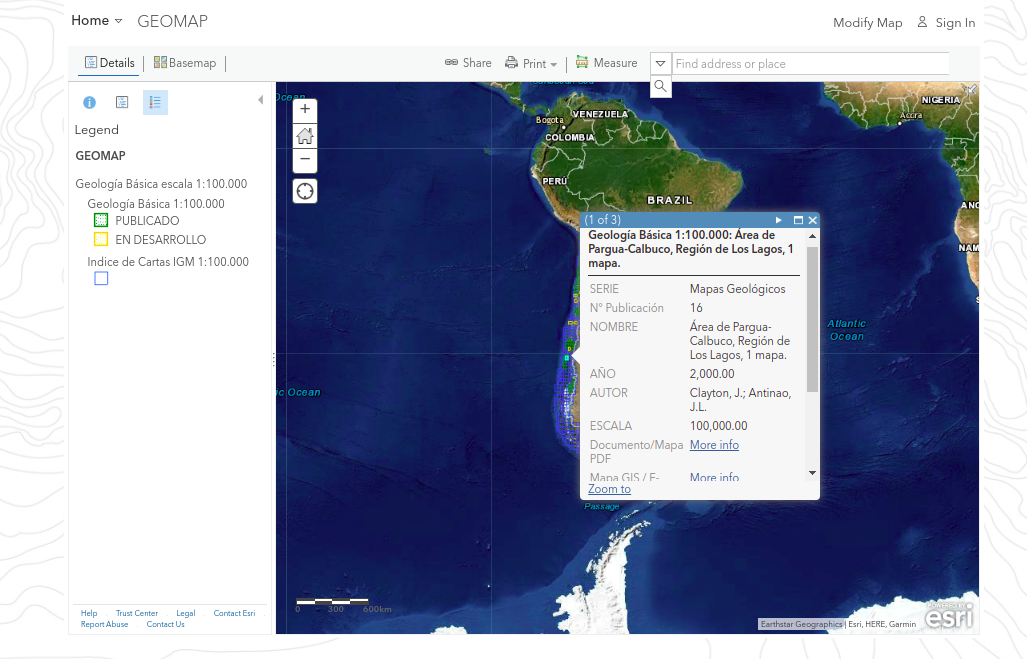
\includegraphics[width=1\textwidth]{images/Contexte/chili.png}
%     \caption{Webmap de SERNAGEOMIN \cite{map2}}
%     \label{fig:chili}
% \end{figure}
